%!TEX root = ../main.tex
%%%%%%%%%%%%%%%%%%%%%%%%%%%%%%%%%%
% Links:
%
% Difficulty:
% Companies: 
%%%%%%%%%%%%%%%%%%%%%%%%%%%%%%%%%%


%\begin{figure}
%	\centering
%	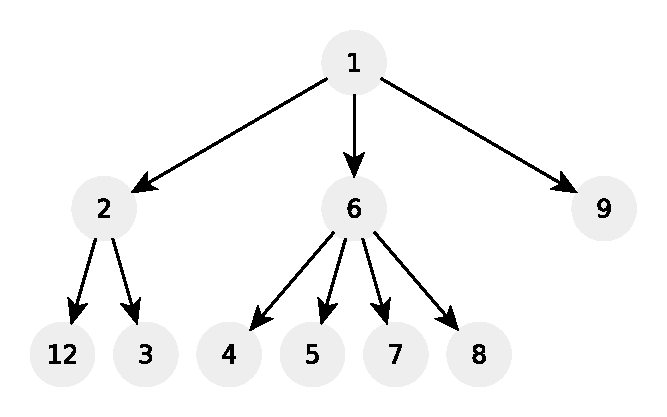
\includegraphics[width=\textwidth]{sources/sort_colors/images/example1}
%	\caption[Sample short cpation]{Sample Caption}.
%	\label{fig:sort_colors:example1}
%\end{figure}

\chapter{Sort the colors}
\label{ch:sort_colors}
\section*{Introduction}

\section{Problem statement}
\begin{exercise}
\label{example:sort_colors:exercice1}
Given an array with n objects colored red, white or blue,
sort them so that objects of the same color are adjacent, with the colors in the order red, white and blue.

Here, we will use the integers 0, 1, and 2 to represent the color red, white, and blue respectively.

Note: Using library sort function is not allowed.

Example :

Input : [0 1 2 0 1 2]
Modify array so that it becomes : [0 0 1 1 2 2]
	%example1
	\begin{example}
		\label{example:sort_colors:example1}
		\hfill \
	}
		
	\end{example}

	%example2
	\begin{example}
		\label{example:sort_colors:example2}
		\hfill \
		
	\end{example}

	\begin{example}
		\hfill \
	
	\label{ex:sort_colors:example3}
	\end{example}

	\begin{example}
		\hfill \

	\label{ex:sort_colors:example4}	
	\end{example}
\end{exercise}

\section{Clarification Questions}

\begin{QandA}
	\item 
	\begin{answered}
		\textit{}
	\end{answered}
	
\end{QandA}

\section{Discussion}
\label{sort_colors:sec:discussion}


\subsection{Brute-force}
\label{sort_colors:sec:bruteforce}

\begin{minipage}{\linewidth}
	\lstinputlisting[language=c++, caption={Sample Caption},label=list:sort_colors]{sources/sort_colors/sort_colors_solution1.cpp}
\end{minipage}

